\chapter{Конструкторская часть}
В данном разделе будут представлены схемы алгоритмов поиска заданного значения в массиве с помощью линейного и двоичного поисков.

\section{Представление алгоритмов}

Алгоритмы на вход получают массив array, значение value, а на выходе возвращают найденный индекс. На рисунках \ref{fig:scheme-1}
--- \ref{fig:scheme-2} представлены схемы алгоритмов.

\begin{figure}[h]
    \centering
    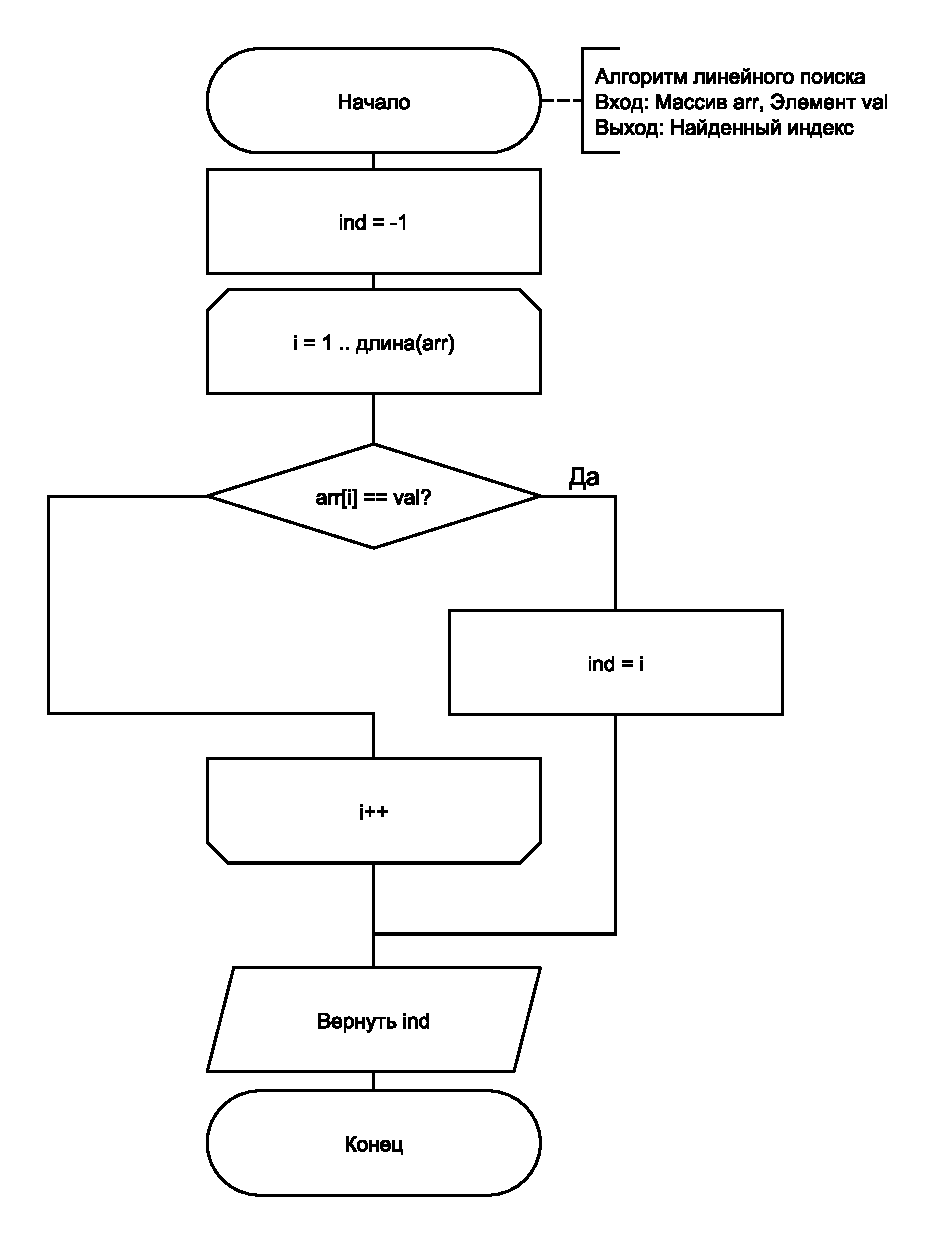
\includegraphics[width=0.8\textwidth]{images/schemes/linear_search.eps}
    \caption{Схема алгоритма поиска в массиве с помощью линейного поиска}
    \label{fig:scheme-1}
\end{figure}

\clearpage

\begin{figure}[h]
    \centering
    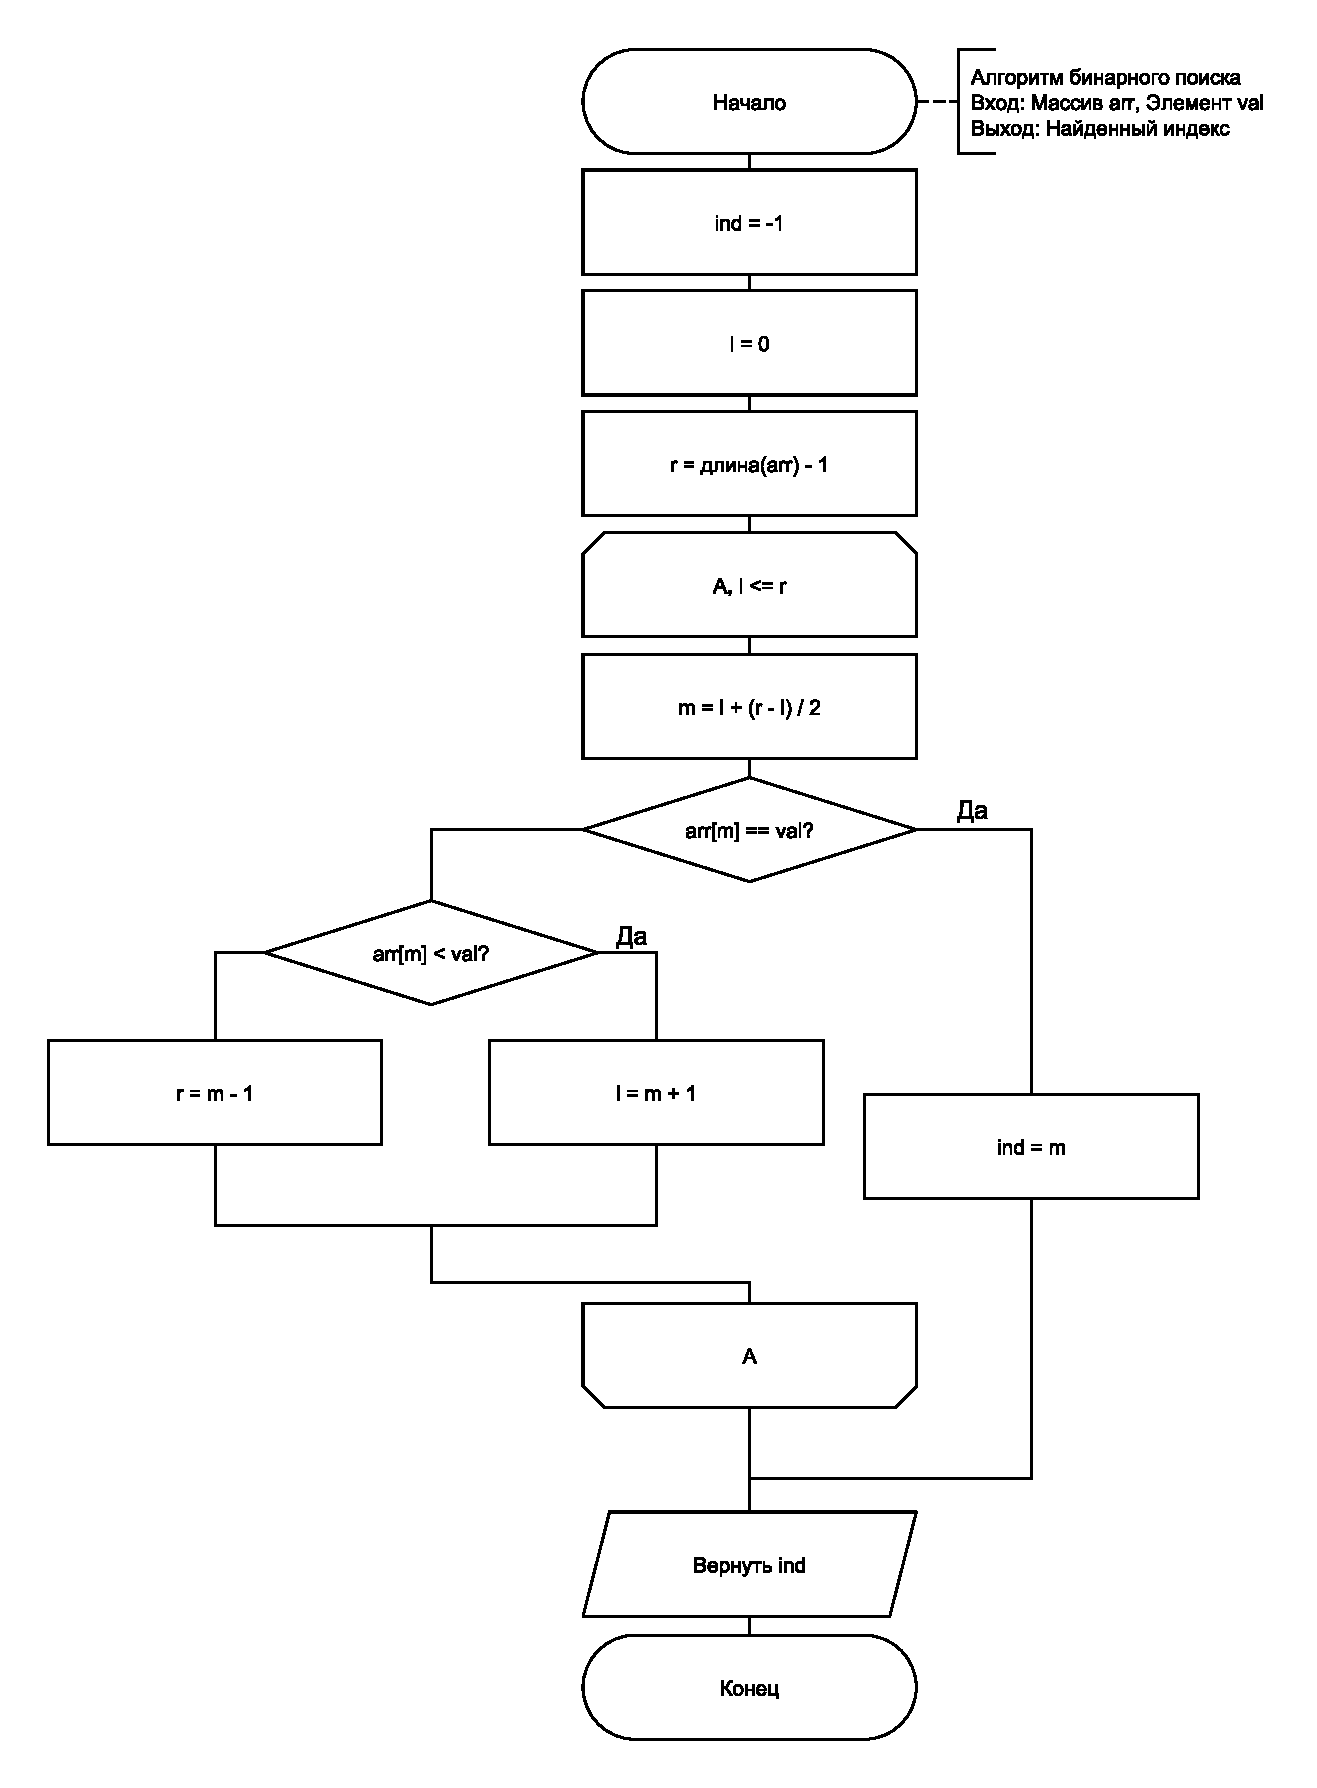
\includegraphics[width=0.8\textwidth]{images/schemes/bin_search.eps}
    \caption{Схема алгоритма поиска в массиве с помощью линейного поиска}
    \label{fig:scheme-2}
\end{figure}

\clearpage

\paragraph*{ВЫВОД} ${}$ \\

В данном разделе были представлены схемы алгоритмов поиска заданного значения в массиве с помощью линейного и двоичного поисков.

\clearpage